\documentclass[twoside]{article}

% Packages required by doxygen
\usepackage{fixltx2e}
\usepackage{calc}
\usepackage{doxygen}
\usepackage{graphicx}
\usepackage[utf8]{inputenc}
\usepackage{makeidx}
\usepackage{multicol}
\usepackage{multirow}
\PassOptionsToPackage{warn}{textcomp}
\usepackage{textcomp}
\usepackage[nointegrals]{wasysym}
\usepackage[table]{xcolor}

% Font selection
\usepackage[T1]{fontenc}
\usepackage{mathptmx}
\usepackage[scaled=.90]{helvet}
\usepackage{courier}
\usepackage{amssymb}
\usepackage{sectsty}
\renewcommand{\familydefault}{\sfdefault}
\allsectionsfont{%
  \fontseries{bc}\selectfont%
  \color{darkgray}%
}
\renewcommand{\DoxyLabelFont}{%
  \fontseries{bc}\selectfont%
  \color{darkgray}%
}
\newcommand{\+}{\discretionary{\mbox{\scriptsize$\hookleftarrow$}}{}{}}

% Page & text layout
\usepackage{geometry}
\geometry{%
  letterpaper,%
  top=2.5cm,%
  bottom=2.5cm,%
  left=2.5cm,%
  right=2.5cm%
}
\tolerance=750
\hfuzz=15pt
\hbadness=750
\setlength{\emergencystretch}{15pt}
\setlength{\parindent}{0cm}
\setlength{\parskip}{0.2cm}
\makeatletter
\renewcommand{\paragraph}{%
  \@startsection{paragraph}{4}{0ex}{-1.0ex}{1.0ex}{%
    \normalfont\normalsize\bfseries\SS@parafont%
  }%
}
\renewcommand{\subparagraph}{%
  \@startsection{subparagraph}{5}{0ex}{-1.0ex}{1.0ex}{%
    \normalfont\normalsize\bfseries\SS@subparafont%
  }%
}
\makeatother

% Headers & footers
\usepackage{fancyhdr}
\pagestyle{fancyplain}
\fancyhead[LE]{\fancyplain{}{\bfseries\thepage}}
\fancyhead[CE]{\fancyplain{}{}}
\fancyhead[RE]{\fancyplain{}{\bfseries\leftmark}}
\fancyhead[LO]{\fancyplain{}{\bfseries\rightmark}}
\fancyhead[CO]{\fancyplain{}{}}
\fancyhead[RO]{\fancyplain{}{\bfseries\thepage}}
\fancyfoot[LE]{\fancyplain{}{}}
\fancyfoot[CE]{\fancyplain{}{}}
\fancyfoot[RE]{\fancyplain{}{\bfseries\scriptsize Generated on Sat Sep 23 2017 00\+:02\+:34 for C\+S124 Lab2 -\/ Linked List Program by Doxygen }}
\fancyfoot[LO]{\fancyplain{}{\bfseries\scriptsize Generated on Sat Sep 23 2017 00\+:02\+:34 for C\+S124 Lab2 -\/ Linked List Program by Doxygen }}
\fancyfoot[CO]{\fancyplain{}{}}
\fancyfoot[RO]{\fancyplain{}{}}
\renewcommand{\footrulewidth}{0.4pt}
\renewcommand{\sectionmark}[1]{%
  \markright{\thesection\ #1}%
}

% Indices & bibliography
\usepackage{natbib}
\usepackage[titles]{tocloft}
\setcounter{tocdepth}{3}
\setcounter{secnumdepth}{5}
\makeindex

% Hyperlinks (required, but should be loaded last)
\usepackage{ifpdf}
\ifpdf
  \usepackage[pdftex,pagebackref=true]{hyperref}
\else
  \usepackage[ps2pdf,pagebackref=true]{hyperref}
\fi
\hypersetup{%
  colorlinks=true,%
  linkcolor=blue,%
  citecolor=blue,%
  unicode%
}

% Custom commands
\newcommand{\clearemptydoublepage}{%
  \newpage{\pagestyle{empty}\cleardoublepage}%
}


%===== C O N T E N T S =====

\begin{document}

% Titlepage & ToC
\hypersetup{pageanchor=false,
             bookmarks=true,
             bookmarksnumbered=true,
             pdfencoding=unicode
            }
\pagenumbering{roman}
\begin{titlepage}
\vspace*{7cm}
\begin{center}%
{\Large C\+S124 Lab2 -\/ Linked List Program }\\
\vspace*{1cm}
{\large Generated by Doxygen 1.8.8}\\
\vspace*{0.5cm}
{\small Sat Sep 23 2017 00:02:34}\\
\end{center}
\end{titlepage}
\tableofcontents
\pagenumbering{arabic}
\hypersetup{pageanchor=true}

%--- Begin generated contents ---
\section{Specification}
\label{Specification}
\hypertarget{Specification}{}
This program has a built in dictionary for english that can be translated to tagalog. It has a user input in which the user may add the translation of a word that is not within the dictionary. 
\section{Analysis}
\label{Analysis}
\hypertarget{Analysis}{}
inputs will be\+:

\begin{DoxyItemize}
\item The outputs will be\+:\end{DoxyItemize}
\begin{DoxyItemize}
\item The overall algorithim is\+: \end{DoxyItemize}

\section{Design}
\label{Design}
\hypertarget{Design}{}
When this program is launched, the user is given the option to choose from any company they would like do their stock exchange. They are given five different companies in a drop down bar to choose from. Once the user has chosen a company, they are given the option to either sell or buy. After the user has chosen one of those two options, the user is then, asked to give their name, shares amount, and price. After the user has entered the following, the program will then execute and insert the information into the heap tree and search through the heap tree. The heap tree will try to find a matching price that the user has input and it will execute the purchase. If there was no match, it will output \char`\"{}\+No seller/buyer\char`\"{} for the user. Also, if the user enter's the name market, it will purchase/sell the shares from the market. After every purchase and sell, it will display in the live graph and live table. The graph and table will update after every transaction. 
\section{1}
\label{Test}
\hypertarget{Test}{}
 
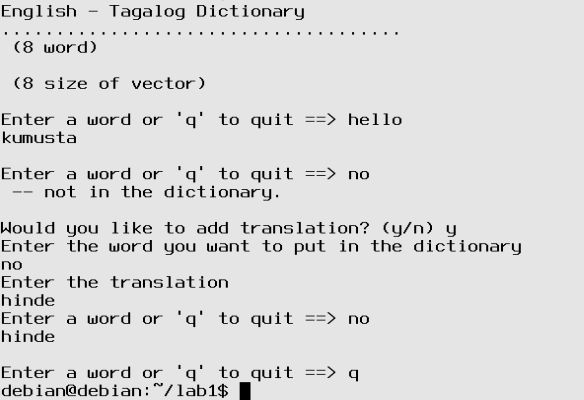
\includegraphics{../lab1.png}
 
\section{Class Index}
\subsection{Class List}
Here are the classes, structs, unions and interfaces with brief descriptions\+:\begin{DoxyCompactList}
\item\contentsline{section}{\hyperlink{structENTRY}{E\+N\+T\+R\+Y} }{\pageref{structENTRY}}{}
\end{DoxyCompactList}

\section{File Index}
\subsection{File List}
Here is a list of all files with brief descriptions\+:\begin{DoxyCompactList}
\item\contentsline{section}{\hyperlink{BuildListDirectly_8cpp}{Build\+List\+Directly.\+cpp} }{\pageref{BuildListDirectly_8cpp}}{}
\item\contentsline{section}{\hyperlink{destroyList_8cpp}{destroy\+List.\+cpp} }{\pageref{destroyList_8cpp}}{}
\item\contentsline{section}{\hyperlink{displayList_8cpp}{display\+List.\+cpp} }{\pageref{displayList_8cpp}}{}
\item\contentsline{section}{\hyperlink{Insert_8cpp}{Insert.\+cpp} }{\pageref{Insert_8cpp}}{}
\item\contentsline{section}{\hyperlink{InsertInOrder_8cpp}{Insert\+In\+Order.\+cpp} }{\pageref{InsertInOrder_8cpp}}{}
\item\contentsline{section}{\hyperlink{lab2_8h}{lab2.\+h} }{\pageref{lab2_8h}}{}
\item\contentsline{section}{\hyperlink{loadList_8cpp}{load\+List.\+cpp} }{\pageref{loadList_8cpp}}{}
\item\contentsline{section}{\hyperlink{loadList2_8cpp}{load\+List2.\+cpp} }{\pageref{loadList2_8cpp}}{}
\item\contentsline{section}{\hyperlink{loadList3_8cpp}{load\+List3.\+cpp} }{\pageref{loadList3_8cpp}}{}
\item\contentsline{section}{\hyperlink{main_8cpp}{main.\+cpp} }{\pageref{main_8cpp}}{}
\end{DoxyCompactList}

\section{Class Documentation}
\hypertarget{structNODE}{\subsection{N\+O\+D\+E Struct Reference}
\label{structNODE}\index{N\+O\+D\+E@{N\+O\+D\+E}}
}


{\ttfamily \#include $<$lab2.\+h$>$}



Collaboration diagram for N\+O\+D\+E\+:\nopagebreak
\begin{figure}[H]
\begin{center}
\leavevmode
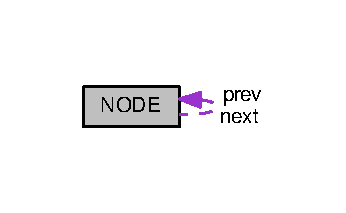
\includegraphics[width=166pt]{structNODE__coll__graph}
\end{center}
\end{figure}
\subsubsection*{Public Attributes}
\begin{DoxyCompactItemize}
\item 
std\+::string \hyperlink{structNODE_a76c9a9603778b363e65bfe84da4bd72e}{city}
\item 
\hyperlink{structNODE}{N\+O\+D\+E} $\ast$ \hyperlink{structNODE_a078472e8ab2d2fe38e052f5c2a425618}{next}
\item 
\hyperlink{structNODE}{N\+O\+D\+E} $\ast$ \hyperlink{structNODE_ab92c64b5b2039998bbf32e9ed3bd55ef}{prev}
\end{DoxyCompactItemize}


\subsubsection{Member Data Documentation}
\hypertarget{structNODE_a76c9a9603778b363e65bfe84da4bd72e}{\index{N\+O\+D\+E@{N\+O\+D\+E}!city@{city}}
\index{city@{city}!N\+O\+D\+E@{N\+O\+D\+E}}
\paragraph[{city}]{\setlength{\rightskip}{0pt plus 5cm}std\+::string N\+O\+D\+E\+::city}}\label{structNODE_a76c9a9603778b363e65bfe84da4bd72e}
\hypertarget{structNODE_a078472e8ab2d2fe38e052f5c2a425618}{\index{N\+O\+D\+E@{N\+O\+D\+E}!next@{next}}
\index{next@{next}!N\+O\+D\+E@{N\+O\+D\+E}}
\paragraph[{next}]{\setlength{\rightskip}{0pt plus 5cm}{\bf N\+O\+D\+E}$\ast$ N\+O\+D\+E\+::next}}\label{structNODE_a078472e8ab2d2fe38e052f5c2a425618}
\hypertarget{structNODE_ab92c64b5b2039998bbf32e9ed3bd55ef}{\index{N\+O\+D\+E@{N\+O\+D\+E}!prev@{prev}}
\index{prev@{prev}!N\+O\+D\+E@{N\+O\+D\+E}}
\paragraph[{prev}]{\setlength{\rightskip}{0pt plus 5cm}{\bf N\+O\+D\+E}$\ast$ N\+O\+D\+E\+::prev}}\label{structNODE_ab92c64b5b2039998bbf32e9ed3bd55ef}


The documentation for this struct was generated from the following file\+:\begin{DoxyCompactItemize}
\item 
\hyperlink{lab2_8h}{lab2.\+h}\end{DoxyCompactItemize}

\section{File Documentation}
\hypertarget{BuildListDirectly_8cpp}{\subsection{Build\+List\+Directly.\+cpp File Reference}
\label{BuildListDirectly_8cpp}\index{Build\+List\+Directly.\+cpp@{Build\+List\+Directly.\+cpp}}
}
{\ttfamily \#include \char`\"{}lab2.\+h\char`\"{}}\\*
Include dependency graph for Build\+List\+Directly.\+cpp\+:\nopagebreak
\begin{figure}[H]
\begin{center}
\leavevmode
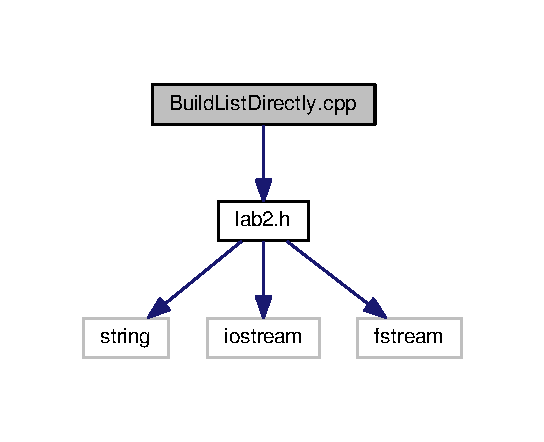
\includegraphics[width=261pt]{BuildListDirectly_8cpp__incl}
\end{center}
\end{figure}
\subsubsection*{Functions}
\begin{DoxyCompactItemize}
\item 
\hyperlink{lab2_8h_a32c27cc471df37f4fc818d65de0a56c4}{S\+T\+A\+T\+U\+S} \hyperlink{BuildListDirectly_8cpp_ab32b9fbd1845e8bb3da2bf84d741ccf3}{Build\+List\+Directly} (\hyperlink{structNODE}{N\+O\+D\+E} $\ast$\&head, std\+::string city)
\begin{DoxyCompactList}\small\item\em Insert the list directly. \end{DoxyCompactList}\end{DoxyCompactItemize}


\subsubsection{Function Documentation}
\hypertarget{BuildListDirectly_8cpp_ab32b9fbd1845e8bb3da2bf84d741ccf3}{\index{Build\+List\+Directly.\+cpp@{Build\+List\+Directly.\+cpp}!Build\+List\+Directly@{Build\+List\+Directly}}
\index{Build\+List\+Directly@{Build\+List\+Directly}!Build\+List\+Directly.\+cpp@{Build\+List\+Directly.\+cpp}}
\paragraph[{Build\+List\+Directly}]{\setlength{\rightskip}{0pt plus 5cm}{\bf S\+T\+A\+T\+U\+S} Build\+List\+Directly (
\begin{DoxyParamCaption}
\item[{{\bf N\+O\+D\+E} $\ast$\&}]{head, }
\item[{std\+::string}]{city}
\end{DoxyParamCaption}
)}}\label{BuildListDirectly_8cpp_ab32b9fbd1845e8bb3da2bf84d741ccf3}


Insert the list directly. 


\begin{DoxyParams}[1]{Parameters}
\mbox{\tt in,out}  & {\em head,Inserting} & the head of linked list, but also called the header //they the same \\
\hline
\mbox{\tt in}  & {\em city,The} & data of the \hyperlink{structNODE}{N\+O\+D\+E} is inserted \\
\hline
\end{DoxyParams}
\begin{DoxyReturn}{Returns}
A S\+T\+A\+T\+U\+S indicating if Build\+List\+Directly was successful or not 
\end{DoxyReturn}

\begin{DoxyCode}
4 \{
5     \hyperlink{structNODE}{NODE} *tail=0, *newnode; \textcolor{comment}{// calls the pointers}
6     head = 0;
7     newnode = \textcolor{keyword}{new} \hyperlink{structNODE}{NODE}; \textcolor{comment}{// allocates a new node}
8     \textcolor{keywordflow}{while} (head != NULL) \textcolor{comment}{//while loop to use link list}
9     \{
10         newnode->\hyperlink{structNODE_a76c9a9603778b363e65bfe84da4bd72e}{city} = city; \textcolor{comment}{//copy list information to newnode}
11         
12     \}
13         newnode->next = 0; \textcolor{comment}{//puts node of next pointer to null}
14         \textcolor{keywordflow}{if} (!tail) \textcolor{comment}{//if it is not tail then head is null}
15             head = newnode;
16         \textcolor{keywordflow}{else}
17             tail->\hyperlink{structNODE_a078472e8ab2d2fe38e052f5c2a425618}{next} = newnode; \textcolor{comment}{//else connect tail with newnode}
18         tail = newnode; \textcolor{comment}{//tail equals to newnode}
19     \textcolor{keywordflow}{return} \hyperlink{lab2_8h_a32c27cc471df37f4fc818d65de0a56c4a2bc49ec37d6a5715dd23e85f1ff5bb59}{OK};
20 \} \textcolor{comment}{//end of function}
\end{DoxyCode}

\hypertarget{destroyList_8cpp}{\subsection{destroy\+List.\+cpp File Reference}
\label{destroyList_8cpp}\index{destroy\+List.\+cpp@{destroy\+List.\+cpp}}
}
{\ttfamily \#include \char`\"{}lab2.\+h\char`\"{}}\\*
Include dependency graph for destroy\+List.\+cpp\+:\nopagebreak
\begin{figure}[H]
\begin{center}
\leavevmode
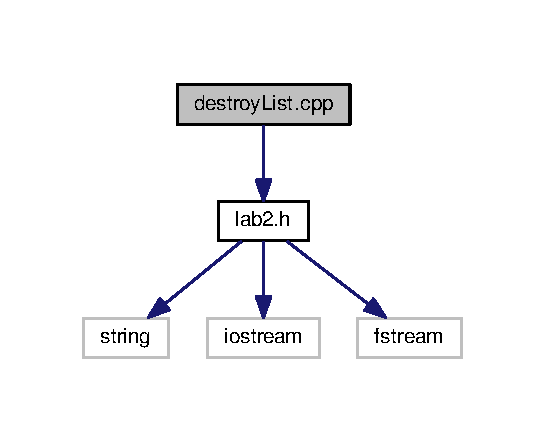
\includegraphics[width=261pt]{destroyList_8cpp__incl}
\end{center}
\end{figure}
\subsubsection*{Functions}
\begin{DoxyCompactItemize}
\item 
void \hyperlink{destroyList_8cpp_ae4c3d5a7f0c1b60f329a966c2e8e9cbd}{destroy\+List} (\hyperlink{structNODE}{N\+O\+D\+E} $\ast$head)
\begin{DoxyCompactList}\small\item\em Destroys the list. \end{DoxyCompactList}\end{DoxyCompactItemize}


\subsubsection{Function Documentation}
\hypertarget{destroyList_8cpp_ae4c3d5a7f0c1b60f329a966c2e8e9cbd}{\index{destroy\+List.\+cpp@{destroy\+List.\+cpp}!destroy\+List@{destroy\+List}}
\index{destroy\+List@{destroy\+List}!destroy\+List.\+cpp@{destroy\+List.\+cpp}}
\paragraph[{destroy\+List}]{\setlength{\rightskip}{0pt plus 5cm}void destroy\+List (
\begin{DoxyParamCaption}
\item[{{\bf N\+O\+D\+E} $\ast$}]{head}
\end{DoxyParamCaption}
)}}\label{destroyList_8cpp_ae4c3d5a7f0c1b60f329a966c2e8e9cbd}


Destroys the list. 


\begin{DoxyParams}{Parameters}
{\em filename} & Name of the file \\
\hline
\end{DoxyParams}
\begin{DoxyReturn}{Returns}
a pointer 'head; to the link list 
\end{DoxyReturn}

\begin{DoxyCode}
4 \{
5     std::cout <<  std::endl; \textcolor{comment}{//to space out lists}
6     \hyperlink{structNODE}{NODE}* node; \textcolor{comment}{//creating node}
7     \textcolor{keywordflow}{for}(node = head; node; node = node->\hyperlink{structNODE_a078472e8ab2d2fe38e052f5c2a425618}{next}) \textcolor{comment}{//loop to delete list}
8     \{       
9             std::cout << \textcolor{stringliteral}{"Deleting: "}
10             << node->\hyperlink{structNODE_a76c9a9603778b363e65bfe84da4bd72e}{city} << std::endl; \textcolor{comment}{// to tell user its deleted}
11             \hyperlink{structNODE}{NODE}* tmp = head->\hyperlink{structNODE_a078472e8ab2d2fe38e052f5c2a425618}{next}; \textcolor{comment}{//assigns head pointer to tmp}
12             \textcolor{comment}{//delete head;}
13             head = tmp; \textcolor{comment}{//head becomes tmp which is deleted}
14 
15     \}
16     
17 \}
\end{DoxyCode}

\hypertarget{displayList_8cpp}{\subsection{display\+List.\+cpp File Reference}
\label{displayList_8cpp}\index{display\+List.\+cpp@{display\+List.\+cpp}}
}
{\ttfamily \#include \char`\"{}lab2.\+h\char`\"{}}\\*
Include dependency graph for display\+List.\+cpp\+:\nopagebreak
\begin{figure}[H]
\begin{center}
\leavevmode
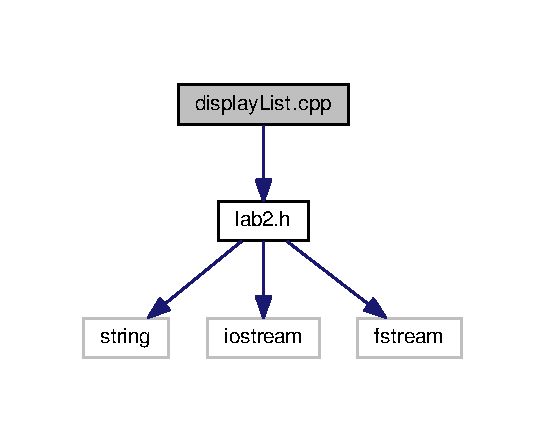
\includegraphics[width=261pt]{displayList_8cpp__incl}
\end{center}
\end{figure}
\subsubsection*{Functions}
\begin{DoxyCompactItemize}
\item 
void \hyperlink{displayList_8cpp_a6d585519d2e25e8317c4939753456dd1}{display\+List} (\hyperlink{structNODE}{N\+O\+D\+E} $\ast$head)
\end{DoxyCompactItemize}


\subsubsection{Function Documentation}
\hypertarget{displayList_8cpp_a6d585519d2e25e8317c4939753456dd1}{\index{display\+List.\+cpp@{display\+List.\+cpp}!display\+List@{display\+List}}
\index{display\+List@{display\+List}!display\+List.\+cpp@{display\+List.\+cpp}}
\paragraph[{display\+List}]{\setlength{\rightskip}{0pt plus 5cm}void display\+List (
\begin{DoxyParamCaption}
\item[{{\bf N\+O\+D\+E} $\ast$}]{head}
\end{DoxyParamCaption}
)}}\label{displayList_8cpp_a6d585519d2e25e8317c4939753456dd1}
This function display th link list 
\begin{DoxyParams}{Parameters}
{\em head} & is a pointer to beginning node of linklist \\
\hline
\end{DoxyParams}
for Node equals head, and node equals node pointing to next, it will print out the city and will continue until it prints out all the list
\begin{DoxyCode}
4 \{   
5     std::cout << \textcolor{stringliteral}{"\(\backslash\)nList: "} << std::endl; \textcolor{comment}{//tells user the list is built}
6     \hyperlink{structNODE}{NODE}* node;
7     \textcolor{keywordflow}{if}(head)
12         \textcolor{keywordflow}{for}(\hyperlink{structNODE}{NODE}* node = head; node; node = node->\hyperlink{structNODE_a078472e8ab2d2fe38e052f5c2a425618}{next})
13         \{    
14             std::cout << node->\hyperlink{structNODE_a76c9a9603778b363e65bfe84da4bd72e}{city} << std::endl;
15         \}
16         \textcolor{keywordflow}{else}
17             std::cout << \textcolor{stringliteral}{"List is empty\(\backslash\)n"} << std::endl;
18             \textcolor{comment}{// if there is nothing in the list, then it will}
19             \textcolor{comment}{//print out this statement}
20 
21 \}
\end{DoxyCode}

\hypertarget{doc_8dox}{\subsection{doc.\+dox File Reference}
\label{doc_8dox}\index{doc.\+dox@{doc.\+dox}}
}

\hypertarget{Insert_8cpp}{\subsection{Insert.\+cpp File Reference}
\label{Insert_8cpp}\index{Insert.\+cpp@{Insert.\+cpp}}
}
{\ttfamily \#include \char`\"{}lab2.\+h\char`\"{}}\\*
Include dependency graph for Insert.\+cpp\+:\nopagebreak
\begin{figure}[H]
\begin{center}
\leavevmode
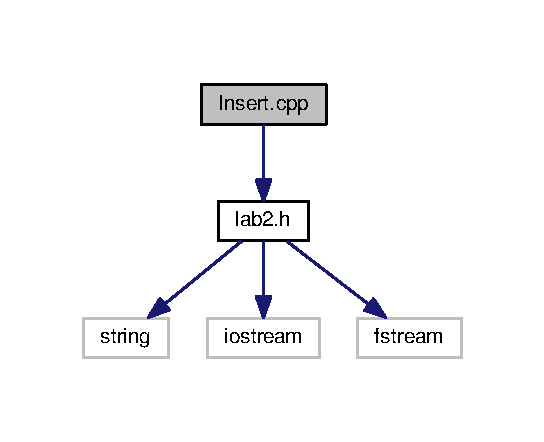
\includegraphics[width=261pt]{Insert_8cpp__incl}
\end{center}
\end{figure}
\subsubsection*{Functions}
\begin{DoxyCompactItemize}
\item 
\hyperlink{lab2_8h_a32c27cc471df37f4fc818d65de0a56c4}{S\+T\+A\+T\+U\+S} \hyperlink{Insert_8cpp_a8b4f4a4d9659ba3856a6272ef31d6e95}{Insert} (\hyperlink{structNODE}{N\+O\+D\+E} $\ast$\&head, std\+::string city)
\begin{DoxyCompactList}\small\item\em Insert puts a new node at the beginning of the list. \end{DoxyCompactList}\end{DoxyCompactItemize}


\subsubsection{Function Documentation}
\hypertarget{Insert_8cpp_a8b4f4a4d9659ba3856a6272ef31d6e95}{\index{Insert.\+cpp@{Insert.\+cpp}!Insert@{Insert}}
\index{Insert@{Insert}!Insert.\+cpp@{Insert.\+cpp}}
\paragraph[{Insert}]{\setlength{\rightskip}{0pt plus 5cm}{\bf S\+T\+A\+T\+U\+S} Insert (
\begin{DoxyParamCaption}
\item[{{\bf N\+O\+D\+E} $\ast$\&}]{head, }
\item[{std\+::string}]{city}
\end{DoxyParamCaption}
)}}\label{Insert_8cpp_a8b4f4a4d9659ba3856a6272ef31d6e95}


Insert puts a new node at the beginning of the list. 


\begin{DoxyParams}[1]{Parameters}
\mbox{\tt in,out}  & {\em head,Inserting} & the head of linked list, but also called the header //they the same \\
\hline
\mbox{\tt in}  & {\em city,The} & data of the \hyperlink{structNODE}{N\+O\+D\+E} is inserted \\
\hline
\end{DoxyParams}
\begin{DoxyReturn}{Returns}
A S\+T\+A\+T\+U\+S indicating if Insert was successful or not A function to insert the linked list into the program which is then printed out for the user 
\end{DoxyReturn}

\begin{DoxyCode}
15 \{
16     \hyperlink{structNODE}{NODE}* newnode = \textcolor{keyword}{new} \hyperlink{structNODE}{NODE}; \textcolor{comment}{//allocating new node}
17     newnode->\hyperlink{structNODE_a76c9a9603778b363e65bfe84da4bd72e}{city} = city; \textcolor{comment}{//copying information into node}
18     newnode->\hyperlink{structNODE_a078472e8ab2d2fe38e052f5c2a425618}{next} = head; \textcolor{comment}{//pointing to head}
19     head = newnode; \textcolor{comment}{//node equals head}
20     \textcolor{keywordflow}{return} \hyperlink{lab2_8h_a32c27cc471df37f4fc818d65de0a56c4a2bc49ec37d6a5715dd23e85f1ff5bb59}{OK};
21 \}
\end{DoxyCode}

\hypertarget{InsertInOrder_8cpp}{\subsection{Insert\+In\+Order.\+cpp File Reference}
\label{InsertInOrder_8cpp}\index{Insert\+In\+Order.\+cpp@{Insert\+In\+Order.\+cpp}}
}
{\ttfamily \#include \char`\"{}lab2.\+h\char`\"{}}\\*
Include dependency graph for Insert\+In\+Order.\+cpp\+:\nopagebreak
\begin{figure}[H]
\begin{center}
\leavevmode
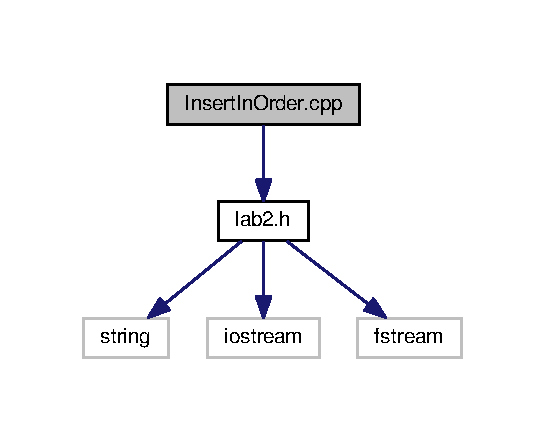
\includegraphics[width=261pt]{InsertInOrder_8cpp__incl}
\end{center}
\end{figure}
\subsubsection*{Functions}
\begin{DoxyCompactItemize}
\item 
\hyperlink{lab2_8h_a32c27cc471df37f4fc818d65de0a56c4}{S\+T\+A\+T\+U\+S} \hyperlink{InsertInOrder_8cpp_afb7f80a286f00ef7b1d83c488097d083}{Insert\+In\+Order} (\hyperlink{structNODE}{N\+O\+D\+E} $\ast$\&head, std\+::string city)
\begin{DoxyCompactList}\small\item\em Insert the list in order. \end{DoxyCompactList}\end{DoxyCompactItemize}


\subsubsection{Function Documentation}
\hypertarget{InsertInOrder_8cpp_afb7f80a286f00ef7b1d83c488097d083}{\index{Insert\+In\+Order.\+cpp@{Insert\+In\+Order.\+cpp}!Insert\+In\+Order@{Insert\+In\+Order}}
\index{Insert\+In\+Order@{Insert\+In\+Order}!Insert\+In\+Order.\+cpp@{Insert\+In\+Order.\+cpp}}
\paragraph[{Insert\+In\+Order}]{\setlength{\rightskip}{0pt plus 5cm}{\bf S\+T\+A\+T\+U\+S} Insert\+In\+Order (
\begin{DoxyParamCaption}
\item[{{\bf N\+O\+D\+E} $\ast$\&}]{head, }
\item[{std\+::string}]{city}
\end{DoxyParamCaption}
)}}\label{InsertInOrder_8cpp_afb7f80a286f00ef7b1d83c488097d083}


Insert the list in order. 

Code that inserts the information of the linked list, but in alphabetical order. 
\begin{DoxyCode}
7 \{
8 
9     \hyperlink{structNODE}{NODE} *newnode; \textcolor{comment}{//creating a new node called newnode}
10     
11     newnode = \textcolor{keyword}{new} \hyperlink{structNODE}{NODE}; \textcolor{comment}{//allocating a new node}
12     \textcolor{keywordflow}{if}(!newnode)
13         \textcolor{keywordflow}{return} \hyperlink{lab2_8h_a32c27cc471df37f4fc818d65de0a56c4aecedb56d1405a60c6069f4a0139bdec5}{FAILED}; \textcolor{comment}{//debugger if it fails}
14         
15     newnode->\hyperlink{structNODE_a76c9a9603778b363e65bfe84da4bd72e}{city}=city; \textcolor{comment}{//to copy information into list}
16     
17     \hyperlink{structNODE}{NODE} *node = head, *prev = 0;
18     \textcolor{comment}{//While node and nodepointing to city is less than}
19     \textcolor{comment}{//or equal to city, prev equals node and node equals}
20     \textcolor{comment}{// node points to next}
21     \textcolor{keywordflow}{while} (node && node->\hyperlink{structNODE_a76c9a9603778b363e65bfe84da4bd72e}{city} <=city)
22     \{
23             prev = node;
24             node = node->\hyperlink{structNODE_a078472e8ab2d2fe38e052f5c2a425618}{next};
25     \}
26     
27     newnode->\hyperlink{structNODE_a078472e8ab2d2fe38e052f5c2a425618}{next} = node;
28     \textcolor{keywordflow}{if}(prev)
29     prev->\hyperlink{structNODE_a078472e8ab2d2fe38e052f5c2a425618}{next} = newnode;
30     \textcolor{keywordflow}{else}
31         head = newnode;
32         
33     \textcolor{keywordflow}{return} \hyperlink{lab2_8h_a32c27cc471df37f4fc818d65de0a56c4a2bc49ec37d6a5715dd23e85f1ff5bb59}{OK};
34         
35 \}
\end{DoxyCode}

\hypertarget{lab2_8h}{\subsection{lab2.\+h File Reference}
\label{lab2_8h}\index{lab2.\+h@{lab2.\+h}}
}
{\ttfamily \#include $<$string$>$}\\*
{\ttfamily \#include $<$iostream$>$}\\*
{\ttfamily \#include $<$fstream$>$}\\*
Include dependency graph for lab2.\+h\+:\nopagebreak
\begin{figure}[H]
\begin{center}
\leavevmode
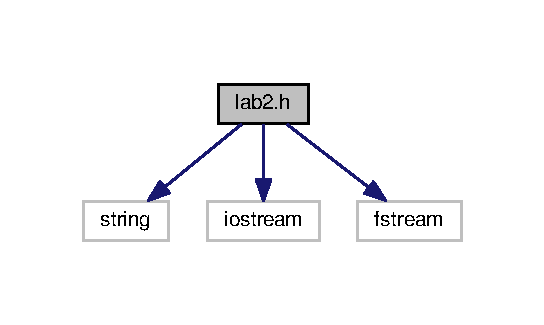
\includegraphics[width=261pt]{lab2_8h__incl}
\end{center}
\end{figure}
This graph shows which files directly or indirectly include this file\+:\nopagebreak
\begin{figure}[H]
\begin{center}
\leavevmode
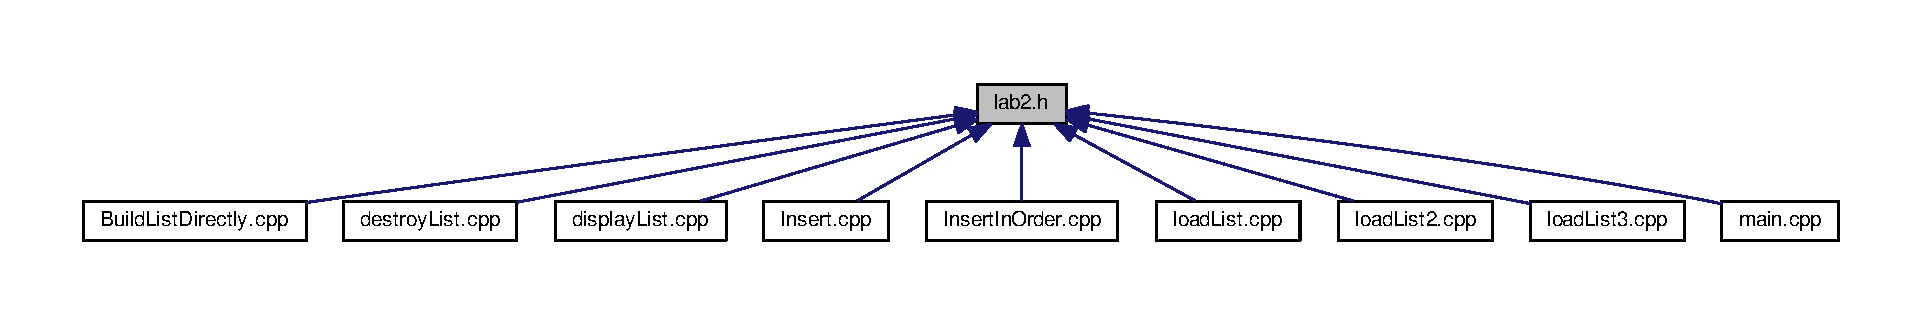
\includegraphics[width=350pt]{lab2_8h__dep__incl}
\end{center}
\end{figure}
\subsubsection*{Classes}
\begin{DoxyCompactItemize}
\item 
struct \hyperlink{structNODE}{N\+O\+D\+E}
\end{DoxyCompactItemize}
\subsubsection*{Enumerations}
\begin{DoxyCompactItemize}
\item 
enum \hyperlink{lab2_8h_a32c27cc471df37f4fc818d65de0a56c4}{S\+T\+A\+T\+U\+S} \{ \hyperlink{lab2_8h_a32c27cc471df37f4fc818d65de0a56c4aecedb56d1405a60c6069f4a0139bdec5}{F\+A\+I\+L\+E\+D}, 
\hyperlink{lab2_8h_a32c27cc471df37f4fc818d65de0a56c4a2bc49ec37d6a5715dd23e85f1ff5bb59}{O\+K}
 \}
\begin{DoxyCompactList}\small\item\em City Structure. \end{DoxyCompactList}\end{DoxyCompactItemize}
\subsubsection*{Functions}
\begin{DoxyCompactItemize}
\item 
\hyperlink{lab2_8h_a32c27cc471df37f4fc818d65de0a56c4}{S\+T\+A\+T\+U\+S} \hyperlink{lab2_8h_a8b4f4a4d9659ba3856a6272ef31d6e95}{Insert} (\hyperlink{structNODE}{N\+O\+D\+E} $\ast$\&head, std\+::string city)
\begin{DoxyCompactList}\small\item\em Insert puts a new node at the beginning of the list. \end{DoxyCompactList}\item 
\hyperlink{structNODE}{N\+O\+D\+E} $\ast$ \hyperlink{lab2_8h_a32d5af33259b5aaf9aa553c5d81049b0}{load\+List} (std\+::string filename)
\begin{DoxyCompactList}\small\item\em This function loads the data from a file. \end{DoxyCompactList}\item 
void \hyperlink{lab2_8h_a6d585519d2e25e8317c4939753456dd1}{display\+List} (\hyperlink{structNODE}{N\+O\+D\+E} $\ast$head)
\item 
void \hyperlink{lab2_8h_ae4c3d5a7f0c1b60f329a966c2e8e9cbd}{destroy\+List} (\hyperlink{structNODE}{N\+O\+D\+E} $\ast$head)
\begin{DoxyCompactList}\small\item\em Destroys the list. \end{DoxyCompactList}\item 
\hyperlink{structNODE}{N\+O\+D\+E} $\ast$ \hyperlink{lab2_8h_aacfafc1182d00a8d4510660bd4190621}{load\+List2} (std\+::string filename)
\begin{DoxyCompactList}\small\item\em This function loads the list in alphabetical order. \end{DoxyCompactList}\item 
\hyperlink{lab2_8h_a32c27cc471df37f4fc818d65de0a56c4}{S\+T\+A\+T\+U\+S} \hyperlink{lab2_8h_afb7f80a286f00ef7b1d83c488097d083}{Insert\+In\+Order} (\hyperlink{structNODE}{N\+O\+D\+E} $\ast$\&head, std\+::string city)
\begin{DoxyCompactList}\small\item\em Insert the list in order. \end{DoxyCompactList}\item 
\hyperlink{structNODE}{N\+O\+D\+E} $\ast$ \hyperlink{lab2_8h_af65c98abd6063427c4a82cc65bb7d813}{load\+List3} (std\+::string filename)
\begin{DoxyCompactList}\small\item\em This function builds the list directly. \end{DoxyCompactList}\item 
\hyperlink{lab2_8h_a32c27cc471df37f4fc818d65de0a56c4}{S\+T\+A\+T\+U\+S} \hyperlink{lab2_8h_ab32b9fbd1845e8bb3da2bf84d741ccf3}{Build\+List\+Directly} (\hyperlink{structNODE}{N\+O\+D\+E} $\ast$\&head, std\+::string city)
\begin{DoxyCompactList}\small\item\em Insert the list directly. \end{DoxyCompactList}\end{DoxyCompactItemize}


\subsubsection{Enumeration Type Documentation}
\hypertarget{lab2_8h_a32c27cc471df37f4fc818d65de0a56c4}{\index{lab2.\+h@{lab2.\+h}!S\+T\+A\+T\+U\+S@{S\+T\+A\+T\+U\+S}}
\index{S\+T\+A\+T\+U\+S@{S\+T\+A\+T\+U\+S}!lab2.\+h@{lab2.\+h}}
\paragraph[{S\+T\+A\+T\+U\+S}]{\setlength{\rightskip}{0pt plus 5cm}enum {\bf S\+T\+A\+T\+U\+S}}}\label{lab2_8h_a32c27cc471df37f4fc818d65de0a56c4}


City Structure. 

This is a structue used to create each node of the linked list of cities enumerate something, number it statuses of new type(string, int, double) \begin{Desc}
\item[Enumerator]\par
\begin{description}
\index{F\+A\+I\+L\+E\+D@{F\+A\+I\+L\+E\+D}!lab2.\+h@{lab2.\+h}}\index{lab2.\+h@{lab2.\+h}!F\+A\+I\+L\+E\+D@{F\+A\+I\+L\+E\+D}}\item[{\em 
\hypertarget{lab2_8h_a32c27cc471df37f4fc818d65de0a56c4aecedb56d1405a60c6069f4a0139bdec5}{F\+A\+I\+L\+E\+D}\label{lab2_8h_a32c27cc471df37f4fc818d65de0a56c4aecedb56d1405a60c6069f4a0139bdec5}
}]\index{O\+K@{O\+K}!lab2.\+h@{lab2.\+h}}\index{lab2.\+h@{lab2.\+h}!O\+K@{O\+K}}\item[{\em 
\hypertarget{lab2_8h_a32c27cc471df37f4fc818d65de0a56c4a2bc49ec37d6a5715dd23e85f1ff5bb59}{O\+K}\label{lab2_8h_a32c27cc471df37f4fc818d65de0a56c4a2bc49ec37d6a5715dd23e85f1ff5bb59}
}]\end{description}
\end{Desc}

\begin{DoxyCode}
16 \{\hyperlink{lab2_8h_a32c27cc471df37f4fc818d65de0a56c4aecedb56d1405a60c6069f4a0139bdec5}{FAILED}, \hyperlink{lab2_8h_a32c27cc471df37f4fc818d65de0a56c4a2bc49ec37d6a5715dd23e85f1ff5bb59}{OK}\};
\end{DoxyCode}


\subsubsection{Function Documentation}
\hypertarget{lab2_8h_ab32b9fbd1845e8bb3da2bf84d741ccf3}{\index{lab2.\+h@{lab2.\+h}!Build\+List\+Directly@{Build\+List\+Directly}}
\index{Build\+List\+Directly@{Build\+List\+Directly}!lab2.\+h@{lab2.\+h}}
\paragraph[{Build\+List\+Directly}]{\setlength{\rightskip}{0pt plus 5cm}{\bf S\+T\+A\+T\+U\+S} Build\+List\+Directly (
\begin{DoxyParamCaption}
\item[{{\bf N\+O\+D\+E} $\ast$\&}]{head, }
\item[{std\+::string}]{city}
\end{DoxyParamCaption}
)}}\label{lab2_8h_ab32b9fbd1845e8bb3da2bf84d741ccf3}


Insert the list directly. 


\begin{DoxyParams}[1]{Parameters}
\mbox{\tt in,out}  & {\em head,Inserting} & the head of linked list, but also called the header //they the same \\
\hline
\mbox{\tt in}  & {\em city,The} & data of the \hyperlink{structNODE}{N\+O\+D\+E} is inserted \\
\hline
\end{DoxyParams}
\begin{DoxyReturn}{Returns}
A S\+T\+A\+T\+U\+S indicating if Build\+List\+Directly was successful or not 
\end{DoxyReturn}

\begin{DoxyCode}
4 \{
5     \hyperlink{structNODE}{NODE} *tail=0, *newnode; \textcolor{comment}{// calls the pointers}
6     head = 0;
7     newnode = \textcolor{keyword}{new} \hyperlink{structNODE}{NODE}; \textcolor{comment}{// allocates a new node}
8     \textcolor{keywordflow}{while} (head != NULL) \textcolor{comment}{//while loop to use link list}
9     \{
10         newnode->\hyperlink{structNODE_a76c9a9603778b363e65bfe84da4bd72e}{city} = city; \textcolor{comment}{//copy list information to newnode}
11         
12     \}
13         newnode->next = 0; \textcolor{comment}{//puts node of next pointer to null}
14         \textcolor{keywordflow}{if} (!tail) \textcolor{comment}{//if it is not tail then head is null}
15             head = newnode;
16         \textcolor{keywordflow}{else}
17             tail->\hyperlink{structNODE_a078472e8ab2d2fe38e052f5c2a425618}{next} = newnode; \textcolor{comment}{//else connect tail with newnode}
18         tail = newnode; \textcolor{comment}{//tail equals to newnode}
19     \textcolor{keywordflow}{return} \hyperlink{lab2_8h_a32c27cc471df37f4fc818d65de0a56c4a2bc49ec37d6a5715dd23e85f1ff5bb59}{OK};
20 \} \textcolor{comment}{//end of function}
\end{DoxyCode}
\hypertarget{lab2_8h_ae4c3d5a7f0c1b60f329a966c2e8e9cbd}{\index{lab2.\+h@{lab2.\+h}!destroy\+List@{destroy\+List}}
\index{destroy\+List@{destroy\+List}!lab2.\+h@{lab2.\+h}}
\paragraph[{destroy\+List}]{\setlength{\rightskip}{0pt plus 5cm}void destroy\+List (
\begin{DoxyParamCaption}
\item[{{\bf N\+O\+D\+E} $\ast$}]{head}
\end{DoxyParamCaption}
)}}\label{lab2_8h_ae4c3d5a7f0c1b60f329a966c2e8e9cbd}


Destroys the list. 


\begin{DoxyParams}{Parameters}
{\em filename} & Name of the file \\
\hline
\end{DoxyParams}
\begin{DoxyReturn}{Returns}
a pointer 'head; to the link list 
\end{DoxyReturn}

\begin{DoxyCode}
4 \{
5     std::cout <<  std::endl; \textcolor{comment}{//to space out lists}
6     \hyperlink{structNODE}{NODE}* node; \textcolor{comment}{//creating node}
7     \textcolor{keywordflow}{for}(node = head; node; node = node->\hyperlink{structNODE_a078472e8ab2d2fe38e052f5c2a425618}{next}) \textcolor{comment}{//loop to delete list}
8     \{       
9             std::cout << \textcolor{stringliteral}{"Deleting: "}
10             << node->\hyperlink{structNODE_a76c9a9603778b363e65bfe84da4bd72e}{city} << std::endl; \textcolor{comment}{// to tell user its deleted}
11             \hyperlink{structNODE}{NODE}* tmp = head->\hyperlink{structNODE_a078472e8ab2d2fe38e052f5c2a425618}{next}; \textcolor{comment}{//assigns head pointer to tmp}
12             \textcolor{comment}{//delete head;}
13             head = tmp; \textcolor{comment}{//head becomes tmp which is deleted}
14 
15     \}
16     
17 \}
\end{DoxyCode}
\hypertarget{lab2_8h_a6d585519d2e25e8317c4939753456dd1}{\index{lab2.\+h@{lab2.\+h}!display\+List@{display\+List}}
\index{display\+List@{display\+List}!lab2.\+h@{lab2.\+h}}
\paragraph[{display\+List}]{\setlength{\rightskip}{0pt plus 5cm}void display\+List (
\begin{DoxyParamCaption}
\item[{{\bf N\+O\+D\+E} $\ast$}]{head}
\end{DoxyParamCaption}
)}}\label{lab2_8h_a6d585519d2e25e8317c4939753456dd1}
This function display th link list 
\begin{DoxyParams}{Parameters}
{\em head} & is a pointer to beginning node of linklist \\
\hline
\end{DoxyParams}
for Node equals head, and node equals node pointing to next, it will print out the city and will continue until it prints out all the list
\begin{DoxyCode}
4 \{   
5     std::cout << \textcolor{stringliteral}{"\(\backslash\)nList: "} << std::endl; \textcolor{comment}{//tells user the list is built}
6     \hyperlink{structNODE}{NODE}* node;
7     \textcolor{keywordflow}{if}(head)
12         \textcolor{keywordflow}{for}(\hyperlink{structNODE}{NODE}* node = head; node; node = node->\hyperlink{structNODE_a078472e8ab2d2fe38e052f5c2a425618}{next})
13         \{    
14             std::cout << node->\hyperlink{structNODE_a76c9a9603778b363e65bfe84da4bd72e}{city} << std::endl;
15         \}
16         \textcolor{keywordflow}{else}
17             std::cout << \textcolor{stringliteral}{"List is empty\(\backslash\)n"} << std::endl;
18             \textcolor{comment}{// if there is nothing in the list, then it will}
19             \textcolor{comment}{//print out this statement}
20 
21 \}
\end{DoxyCode}
\hypertarget{lab2_8h_a8b4f4a4d9659ba3856a6272ef31d6e95}{\index{lab2.\+h@{lab2.\+h}!Insert@{Insert}}
\index{Insert@{Insert}!lab2.\+h@{lab2.\+h}}
\paragraph[{Insert}]{\setlength{\rightskip}{0pt plus 5cm}{\bf S\+T\+A\+T\+U\+S} Insert (
\begin{DoxyParamCaption}
\item[{{\bf N\+O\+D\+E} $\ast$\&}]{head, }
\item[{std\+::string}]{city}
\end{DoxyParamCaption}
)}}\label{lab2_8h_a8b4f4a4d9659ba3856a6272ef31d6e95}


Insert puts a new node at the beginning of the list. 


\begin{DoxyParams}[1]{Parameters}
\mbox{\tt in,out}  & {\em head,Inserting} & the head of linked list, but also called the header //they the same \\
\hline
\mbox{\tt in}  & {\em city,The} & data of the \hyperlink{structNODE}{N\+O\+D\+E} is inserted \\
\hline
\end{DoxyParams}
\begin{DoxyReturn}{Returns}
A S\+T\+A\+T\+U\+S indicating if Insert was successful or not
\end{DoxyReturn}

\begin{DoxyParams}[1]{Parameters}
\mbox{\tt in,out}  & {\em head,Inserting} & the head of linked list, but also called the header //they the same \\
\hline
\mbox{\tt in}  & {\em city,The} & data of the \hyperlink{structNODE}{N\+O\+D\+E} is inserted \\
\hline
\end{DoxyParams}
\begin{DoxyReturn}{Returns}
A S\+T\+A\+T\+U\+S indicating if Insert was successful or not A function to insert the linked list into the program which is then printed out for the user 
\end{DoxyReturn}

\begin{DoxyCode}
15 \{
16     \hyperlink{structNODE}{NODE}* newnode = \textcolor{keyword}{new} \hyperlink{structNODE}{NODE}; \textcolor{comment}{//allocating new node}
17     newnode->\hyperlink{structNODE_a76c9a9603778b363e65bfe84da4bd72e}{city} = city; \textcolor{comment}{//copying information into node}
18     newnode->\hyperlink{structNODE_a078472e8ab2d2fe38e052f5c2a425618}{next} = head; \textcolor{comment}{//pointing to head}
19     head = newnode; \textcolor{comment}{//node equals head}
20     \textcolor{keywordflow}{return} \hyperlink{lab2_8h_a32c27cc471df37f4fc818d65de0a56c4a2bc49ec37d6a5715dd23e85f1ff5bb59}{OK};
21 \}
\end{DoxyCode}
\hypertarget{lab2_8h_afb7f80a286f00ef7b1d83c488097d083}{\index{lab2.\+h@{lab2.\+h}!Insert\+In\+Order@{Insert\+In\+Order}}
\index{Insert\+In\+Order@{Insert\+In\+Order}!lab2.\+h@{lab2.\+h}}
\paragraph[{Insert\+In\+Order}]{\setlength{\rightskip}{0pt plus 5cm}{\bf S\+T\+A\+T\+U\+S} Insert\+In\+Order (
\begin{DoxyParamCaption}
\item[{{\bf N\+O\+D\+E} $\ast$\&}]{head, }
\item[{std\+::string}]{city}
\end{DoxyParamCaption}
)}}\label{lab2_8h_afb7f80a286f00ef7b1d83c488097d083}


Insert the list in order. 


\begin{DoxyParams}[1]{Parameters}
\mbox{\tt in,out}  & {\em head,Inserting} & the head of linked list, but also called the header //they the same \\
\hline
\mbox{\tt in}  & {\em city,The} & data of the \hyperlink{structNODE}{N\+O\+D\+E} is inserted \\
\hline
\end{DoxyParams}
\begin{DoxyReturn}{Returns}
A S\+T\+A\+T\+U\+S indicating if Insert was successful or not
\end{DoxyReturn}
Code that inserts the information of the linked list, but in alphabetical order. 
\begin{DoxyCode}
7 \{
8 
9     \hyperlink{structNODE}{NODE} *newnode; \textcolor{comment}{//creating a new node called newnode}
10     
11     newnode = \textcolor{keyword}{new} \hyperlink{structNODE}{NODE}; \textcolor{comment}{//allocating a new node}
12     \textcolor{keywordflow}{if}(!newnode)
13         \textcolor{keywordflow}{return} \hyperlink{lab2_8h_a32c27cc471df37f4fc818d65de0a56c4aecedb56d1405a60c6069f4a0139bdec5}{FAILED}; \textcolor{comment}{//debugger if it fails}
14         
15     newnode->\hyperlink{structNODE_a76c9a9603778b363e65bfe84da4bd72e}{city}=city; \textcolor{comment}{//to copy information into list}
16     
17     \hyperlink{structNODE}{NODE} *node = head, *prev = 0;
18     \textcolor{comment}{//While node and nodepointing to city is less than}
19     \textcolor{comment}{//or equal to city, prev equals node and node equals}
20     \textcolor{comment}{// node points to next}
21     \textcolor{keywordflow}{while} (node && node->\hyperlink{structNODE_a76c9a9603778b363e65bfe84da4bd72e}{city} <=city)
22     \{
23             prev = node;
24             node = node->\hyperlink{structNODE_a078472e8ab2d2fe38e052f5c2a425618}{next};
25     \}
26     
27     newnode->\hyperlink{structNODE_a078472e8ab2d2fe38e052f5c2a425618}{next} = node;
28     \textcolor{keywordflow}{if}(prev)
29     prev->\hyperlink{structNODE_a078472e8ab2d2fe38e052f5c2a425618}{next} = newnode;
30     \textcolor{keywordflow}{else}
31         head = newnode;
32         
33     \textcolor{keywordflow}{return} \hyperlink{lab2_8h_a32c27cc471df37f4fc818d65de0a56c4a2bc49ec37d6a5715dd23e85f1ff5bb59}{OK};
34         
35 \}
\end{DoxyCode}
\hypertarget{lab2_8h_a32d5af33259b5aaf9aa553c5d81049b0}{\index{lab2.\+h@{lab2.\+h}!load\+List@{load\+List}}
\index{load\+List@{load\+List}!lab2.\+h@{lab2.\+h}}
\paragraph[{load\+List}]{\setlength{\rightskip}{0pt plus 5cm}{\bf N\+O\+D\+E}$\ast$ load\+List (
\begin{DoxyParamCaption}
\item[{std\+::string}]{filename}
\end{DoxyParamCaption}
)}}\label{lab2_8h_a32d5af33259b5aaf9aa553c5d81049b0}


This function loads the data from a file. 

The file contains a list of cities, each on a seperate line. 
\begin{DoxyParams}{Parameters}
{\em filename} & Name of file \\
\hline
\end{DoxyParams}
\begin{DoxyReturn}{Returns}
a pointer 'head' to the link list
\end{DoxyReturn}

\begin{DoxyImage}
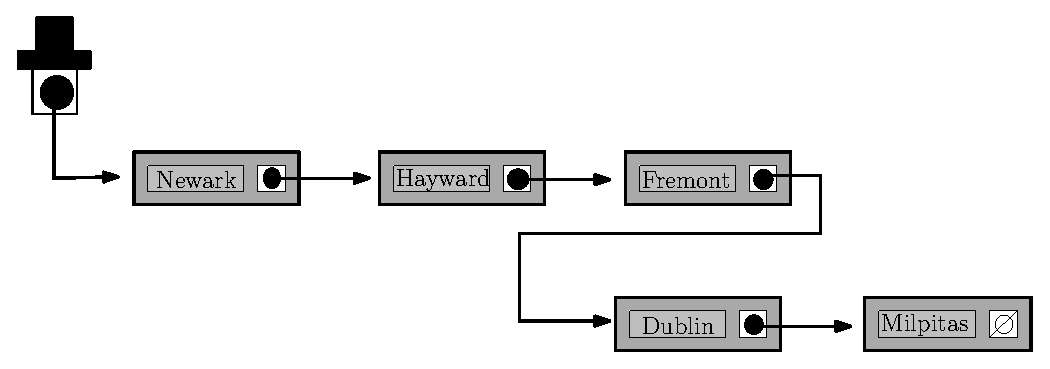
\includegraphics{./lab2fig1}
\caption{Linked List}
\end{DoxyImage}
loads the linked list into the program which lets the function Display\+List print it out for the user 
\begin{DoxyCode}
10 \{
11     \hyperlink{structNODE}{NODE}* head = 0; \textcolor{comment}{//puts head to null}
12     std::ifstream inputFile(filename.c\_str()); \textcolor{comment}{//taking input}
13     std::string city; \textcolor{comment}{//to use string city for list}
14     \textcolor{keywordflow}{while} (inputFile >> city) \textcolor{comment}{// loop to grab information}
15         \textcolor{keywordflow}{if} (\hyperlink{Insert_8cpp_a8b4f4a4d9659ba3856a6272ef31d6e95}{Insert}(head, city) == \hyperlink{lab2_8h_a32c27cc471df37f4fc818d65de0a56c4aecedb56d1405a60c6069f4a0139bdec5}{FAILED})
16             std::cerr << \textcolor{stringliteral}{"Error on Insert\(\backslash\)n"};
17         \textcolor{comment}{//if statements that catches error if it cannot}
18         \textcolor{comment}{//get linked list information}
19     \textcolor{keywordflow}{return} head; \textcolor{comment}{//returns head}
20 \}
\end{DoxyCode}
\hypertarget{lab2_8h_aacfafc1182d00a8d4510660bd4190621}{\index{lab2.\+h@{lab2.\+h}!load\+List2@{load\+List2}}
\index{load\+List2@{load\+List2}!lab2.\+h@{lab2.\+h}}
\paragraph[{load\+List2}]{\setlength{\rightskip}{0pt plus 5cm}{\bf N\+O\+D\+E}$\ast$ load\+List2 (
\begin{DoxyParamCaption}
\item[{std\+::string}]{filename}
\end{DoxyParamCaption}
)}}\label{lab2_8h_aacfafc1182d00a8d4510660bd4190621}


This function loads the list in alphabetical order. 

The file contains a list of cities, each on a seperate line. 
\begin{DoxyParams}{Parameters}
{\em filename} & Name of file \\
\hline
\end{DoxyParams}
\begin{DoxyReturn}{Returns}
a pointer 'head' to the link list
\end{DoxyReturn}

\begin{DoxyImage}
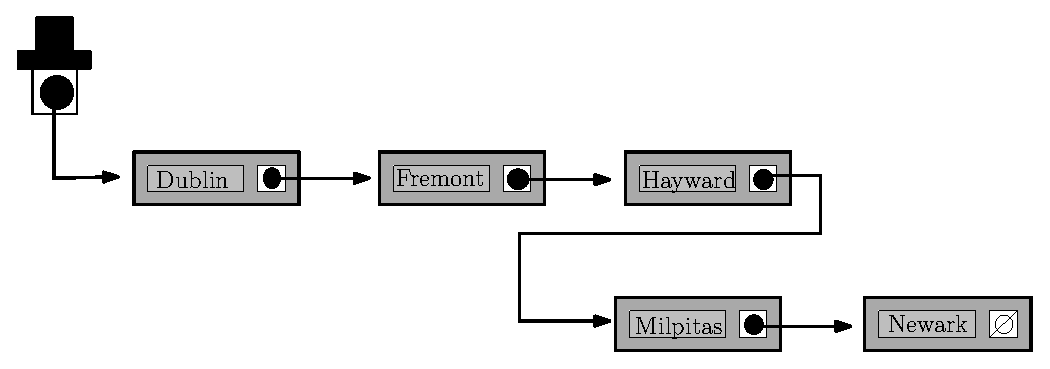
\includegraphics{./lab2fig2}
\caption{Linked List}
\end{DoxyImage}

\begin{DoxyCode}
6 \{
7     \hyperlink{structNODE}{NODE}* head = 0; \textcolor{comment}{//puts head to null}
8     std::ifstream inputFile(filename.c\_str()); \textcolor{comment}{//taking input}
9     std::string city; \textcolor{comment}{//to use string city for list}
10     \textcolor{keywordflow}{while} (inputFile >> city) \textcolor{comment}{// loop to grab information}
11         \textcolor{keywordflow}{if} (\hyperlink{InsertInOrder_8cpp_afb7f80a286f00ef7b1d83c488097d083}{InsertInOrder}(head, city) == \hyperlink{lab2_8h_a32c27cc471df37f4fc818d65de0a56c4aecedb56d1405a60c6069f4a0139bdec5}{FAILED})
12             std::cerr << \textcolor{stringliteral}{"Error on Insert\(\backslash\)n"};
13             \textcolor{comment}{//if statements that catches error if it cannot}
14         \textcolor{comment}{//get linked list information}
15     \textcolor{keywordflow}{return} head; \textcolor{comment}{//returns head}
16 \}
\end{DoxyCode}
\hypertarget{lab2_8h_af65c98abd6063427c4a82cc65bb7d813}{\index{lab2.\+h@{lab2.\+h}!load\+List3@{load\+List3}}
\index{load\+List3@{load\+List3}!lab2.\+h@{lab2.\+h}}
\paragraph[{load\+List3}]{\setlength{\rightskip}{0pt plus 5cm}{\bf N\+O\+D\+E}$\ast$ load\+List3 (
\begin{DoxyParamCaption}
\item[{std\+::string}]{filename}
\end{DoxyParamCaption}
)}}\label{lab2_8h_af65c98abd6063427c4a82cc65bb7d813}


This function builds the list directly. 

The file contains a list of cities, each on a seperate line. 
\begin{DoxyParams}{Parameters}
{\em filename} & Name of file \\
\hline
\end{DoxyParams}
\begin{DoxyReturn}{Returns}
a pointer 'head' and also a pointer 'tail' to the link list
\end{DoxyReturn}

\begin{DoxyImage}
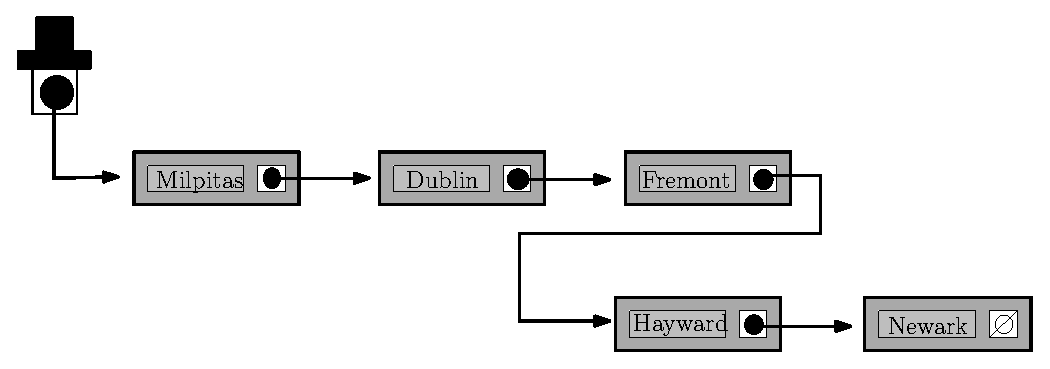
\includegraphics{./lab2fig3}
\caption{Linked List}
\end{DoxyImage}

\begin{DoxyCode}
6 \{
7     \hyperlink{structNODE}{NODE}* head = 0;  \textcolor{comment}{//puts head to null}
8     std::ifstream inputFile(filename.c\_str()); \textcolor{comment}{//taking input}
9     std::string city; \textcolor{comment}{//to use string city for list}
10     \textcolor{keywordflow}{while} (inputFile >> city) \textcolor{comment}{// loop to grab information}
11         \textcolor{keywordflow}{if} (\hyperlink{BuildListDirectly_8cpp_ab32b9fbd1845e8bb3da2bf84d741ccf3}{BuildListDirectly}(head, city) == \hyperlink{lab2_8h_a32c27cc471df37f4fc818d65de0a56c4aecedb56d1405a60c6069f4a0139bdec5}{FAILED})
12             std::cerr << \textcolor{stringliteral}{"Error on Insert\(\backslash\)n"};
13             \textcolor{comment}{//if statements that catches error if it cannot}
14         \textcolor{comment}{//get linked list information}
15     \textcolor{keywordflow}{return} head; \textcolor{comment}{//returns head}
16 \}
\end{DoxyCode}

\hypertarget{loadList_8cpp}{\subsection{load\+List.\+cpp File Reference}
\label{loadList_8cpp}\index{load\+List.\+cpp@{load\+List.\+cpp}}
}
{\ttfamily \#include \char`\"{}lab2.\+h\char`\"{}}\\*
Include dependency graph for load\+List.\+cpp\+:\nopagebreak
\begin{figure}[H]
\begin{center}
\leavevmode
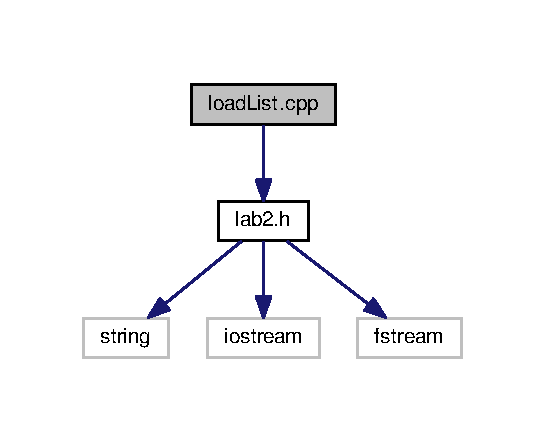
\includegraphics[width=261pt]{loadList_8cpp__incl}
\end{center}
\end{figure}
\subsubsection*{Functions}
\begin{DoxyCompactItemize}
\item 
\hyperlink{structNODE}{N\+O\+D\+E} $\ast$ \hyperlink{loadList_8cpp_a32d5af33259b5aaf9aa553c5d81049b0}{load\+List} (std\+::string filename)
\begin{DoxyCompactList}\small\item\em This function loads the data from a file. \end{DoxyCompactList}\end{DoxyCompactItemize}


\subsubsection{Function Documentation}
\hypertarget{loadList_8cpp_a32d5af33259b5aaf9aa553c5d81049b0}{\index{load\+List.\+cpp@{load\+List.\+cpp}!load\+List@{load\+List}}
\index{load\+List@{load\+List}!load\+List.\+cpp@{load\+List.\+cpp}}
\paragraph[{load\+List}]{\setlength{\rightskip}{0pt plus 5cm}{\bf N\+O\+D\+E}$\ast$ load\+List (
\begin{DoxyParamCaption}
\item[{std\+::string}]{filename}
\end{DoxyParamCaption}
)}}\label{loadList_8cpp_a32d5af33259b5aaf9aa553c5d81049b0}


This function loads the data from a file. 


\begin{DoxyImage}
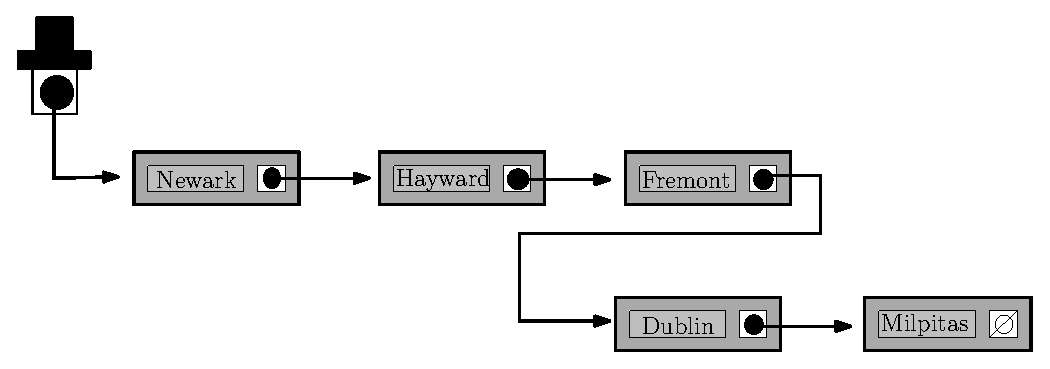
\includegraphics{./lab2fig1}
\caption{Linked List}
\end{DoxyImage}
loads the linked list into the program which lets the function Display\+List print it out for the user 
\begin{DoxyCode}
10 \{
11     \hyperlink{structNODE}{NODE}* head = 0; \textcolor{comment}{//puts head to null}
12     std::ifstream inputFile(filename.c\_str()); \textcolor{comment}{//taking input}
13     std::string city; \textcolor{comment}{//to use string city for list}
14     \textcolor{keywordflow}{while} (inputFile >> city) \textcolor{comment}{// loop to grab information}
15         \textcolor{keywordflow}{if} (\hyperlink{Insert_8cpp_a8b4f4a4d9659ba3856a6272ef31d6e95}{Insert}(head, city) == \hyperlink{lab2_8h_a32c27cc471df37f4fc818d65de0a56c4aecedb56d1405a60c6069f4a0139bdec5}{FAILED})
16             std::cerr << \textcolor{stringliteral}{"Error on Insert\(\backslash\)n"};
17         \textcolor{comment}{//if statements that catches error if it cannot}
18         \textcolor{comment}{//get linked list information}
19     \textcolor{keywordflow}{return} head; \textcolor{comment}{//returns head}
20 \}
\end{DoxyCode}

\hypertarget{loadList2_8cpp}{\subsection{load\+List2.\+cpp File Reference}
\label{loadList2_8cpp}\index{load\+List2.\+cpp@{load\+List2.\+cpp}}
}
{\ttfamily \#include \char`\"{}lab2.\+h\char`\"{}}\\*
Include dependency graph for load\+List2.\+cpp\+:\nopagebreak
\begin{figure}[H]
\begin{center}
\leavevmode
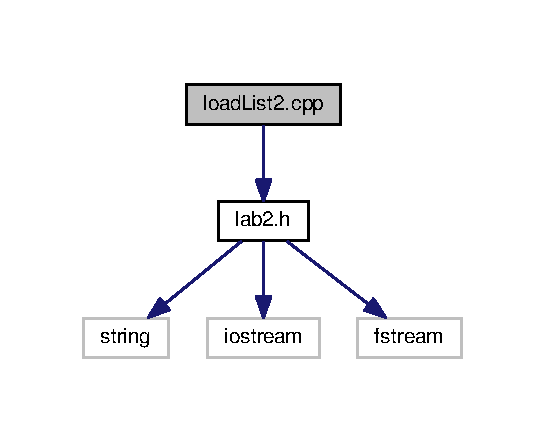
\includegraphics[width=261pt]{loadList2_8cpp__incl}
\end{center}
\end{figure}
\subsubsection*{Functions}
\begin{DoxyCompactItemize}
\item 
\hyperlink{structNODE}{N\+O\+D\+E} $\ast$ \hyperlink{loadList2_8cpp_aacfafc1182d00a8d4510660bd4190621}{load\+List2} (std\+::string filename)
\begin{DoxyCompactList}\small\item\em This function loads the list in alphabetical order. \end{DoxyCompactList}\end{DoxyCompactItemize}


\subsubsection{Function Documentation}
\hypertarget{loadList2_8cpp_aacfafc1182d00a8d4510660bd4190621}{\index{load\+List2.\+cpp@{load\+List2.\+cpp}!load\+List2@{load\+List2}}
\index{load\+List2@{load\+List2}!load\+List2.\+cpp@{load\+List2.\+cpp}}
\paragraph[{load\+List2}]{\setlength{\rightskip}{0pt plus 5cm}{\bf N\+O\+D\+E}$\ast$ load\+List2 (
\begin{DoxyParamCaption}
\item[{std\+::string}]{filename}
\end{DoxyParamCaption}
)}}\label{loadList2_8cpp_aacfafc1182d00a8d4510660bd4190621}


This function loads the list in alphabetical order. 


\begin{DoxyImage}
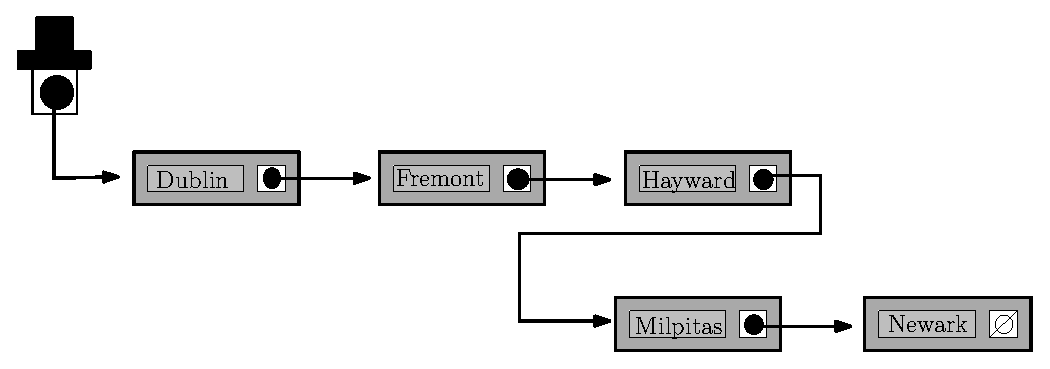
\includegraphics{./lab2fig2}
\caption{Linked List}
\end{DoxyImage}

\begin{DoxyCode}
6 \{
7     \hyperlink{structNODE}{NODE}* head = 0; \textcolor{comment}{//puts head to null}
8     std::ifstream inputFile(filename.c\_str()); \textcolor{comment}{//taking input}
9     std::string city; \textcolor{comment}{//to use string city for list}
10     \textcolor{keywordflow}{while} (inputFile >> city) \textcolor{comment}{// loop to grab information}
11         \textcolor{keywordflow}{if} (\hyperlink{InsertInOrder_8cpp_afb7f80a286f00ef7b1d83c488097d083}{InsertInOrder}(head, city) == \hyperlink{lab2_8h_a32c27cc471df37f4fc818d65de0a56c4aecedb56d1405a60c6069f4a0139bdec5}{FAILED})
12             std::cerr << \textcolor{stringliteral}{"Error on Insert\(\backslash\)n"};
13             \textcolor{comment}{//if statements that catches error if it cannot}
14         \textcolor{comment}{//get linked list information}
15     \textcolor{keywordflow}{return} head; \textcolor{comment}{//returns head}
16 \}
\end{DoxyCode}

\hypertarget{loadList3_8cpp}{\subsection{load\+List3.\+cpp File Reference}
\label{loadList3_8cpp}\index{load\+List3.\+cpp@{load\+List3.\+cpp}}
}
{\ttfamily \#include \char`\"{}lab2.\+h\char`\"{}}\\*
Include dependency graph for load\+List3.\+cpp\+:\nopagebreak
\begin{figure}[H]
\begin{center}
\leavevmode
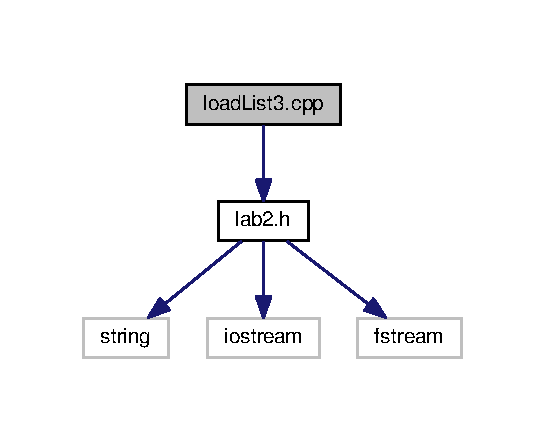
\includegraphics[width=261pt]{loadList3_8cpp__incl}
\end{center}
\end{figure}
\subsubsection*{Functions}
\begin{DoxyCompactItemize}
\item 
\hyperlink{structNODE}{N\+O\+D\+E} $\ast$ \hyperlink{loadList3_8cpp_af65c98abd6063427c4a82cc65bb7d813}{load\+List3} (std\+::string filename)
\begin{DoxyCompactList}\small\item\em This function builds the list directly. \end{DoxyCompactList}\end{DoxyCompactItemize}


\subsubsection{Function Documentation}
\hypertarget{loadList3_8cpp_af65c98abd6063427c4a82cc65bb7d813}{\index{load\+List3.\+cpp@{load\+List3.\+cpp}!load\+List3@{load\+List3}}
\index{load\+List3@{load\+List3}!load\+List3.\+cpp@{load\+List3.\+cpp}}
\paragraph[{load\+List3}]{\setlength{\rightskip}{0pt plus 5cm}{\bf N\+O\+D\+E}$\ast$ load\+List3 (
\begin{DoxyParamCaption}
\item[{std\+::string}]{filename}
\end{DoxyParamCaption}
)}}\label{loadList3_8cpp_af65c98abd6063427c4a82cc65bb7d813}


This function builds the list directly. 


\begin{DoxyImage}
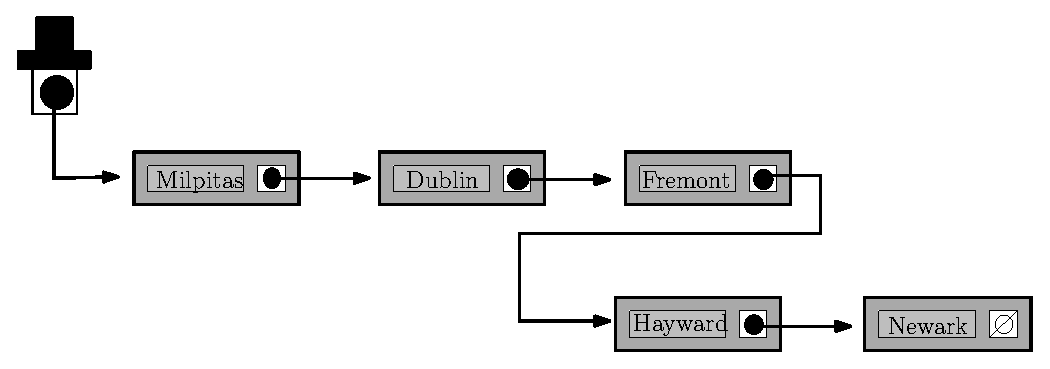
\includegraphics{./lab2fig3}
\caption{Linked List}
\end{DoxyImage}

\begin{DoxyCode}
6 \{
7     \hyperlink{structNODE}{NODE}* head = 0;  \textcolor{comment}{//puts head to null}
8     std::ifstream inputFile(filename.c\_str()); \textcolor{comment}{//taking input}
9     std::string city; \textcolor{comment}{//to use string city for list}
10     \textcolor{keywordflow}{while} (inputFile >> city) \textcolor{comment}{// loop to grab information}
11         \textcolor{keywordflow}{if} (\hyperlink{BuildListDirectly_8cpp_ab32b9fbd1845e8bb3da2bf84d741ccf3}{BuildListDirectly}(head, city) == \hyperlink{lab2_8h_a32c27cc471df37f4fc818d65de0a56c4aecedb56d1405a60c6069f4a0139bdec5}{FAILED})
12             std::cerr << \textcolor{stringliteral}{"Error on Insert\(\backslash\)n"};
13             \textcolor{comment}{//if statements that catches error if it cannot}
14         \textcolor{comment}{//get linked list information}
15     \textcolor{keywordflow}{return} head; \textcolor{comment}{//returns head}
16 \}
\end{DoxyCode}

\hypertarget{main_8cpp}{\subsection{main.\+cpp File Reference}
\label{main_8cpp}\index{main.\+cpp@{main.\+cpp}}
}
{\ttfamily \#include \char`\"{}lab.\+h\char`\"{}}\\*
Include dependency graph for main.\+cpp\+:\nopagebreak
\begin{figure}[H]
\begin{center}
\leavevmode
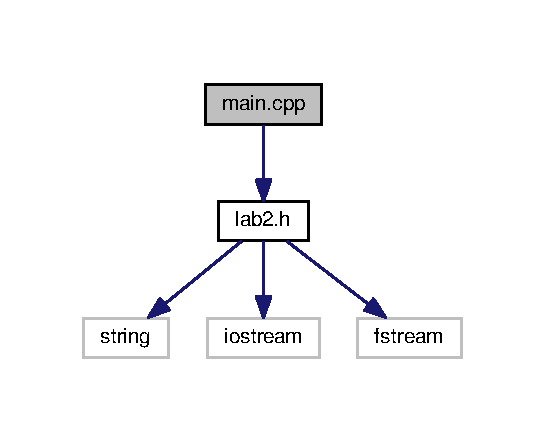
\includegraphics[width=350pt]{main_8cpp__incl}
\end{center}
\end{figure}
\subsubsection*{Functions}
\begin{DoxyCompactItemize}
\item 
int \hyperlink{main_8cpp_ae66f6b31b5ad750f1fe042a706a4e3d4}{main} ()
\end{DoxyCompactItemize}
\subsubsection*{Variables}
\begin{DoxyCompactItemize}
\item 
Fl\+\_\+\+Input $\ast$ \hyperlink{main_8cpp_abf805c82a90897837d1c26ef915f1cd6}{pizza}
\item 
Fl\+\_\+\+Output $\ast$ \hyperlink{main_8cpp_a05c7f6e86cca5f4d0ebf44d1f5042c37}{watch}
\item 
Fl\+\_\+\+Text\+\_\+\+Buffer $\ast$ \hyperlink{main_8cpp_aea2b8efadc87a819fe57c311d668e504}{buff}
\item 
Fl\+\_\+\+Text\+\_\+\+Display $\ast$ \hyperlink{main_8cpp_a23f917547a833922fd6bc8797cc04ee1}{order\+Q}
\end{DoxyCompactItemize}


\subsubsection{Function Documentation}
\hypertarget{main_8cpp_ae66f6b31b5ad750f1fe042a706a4e3d4}{\index{main.\+cpp@{main.\+cpp}!main@{main}}
\index{main@{main}!main.\+cpp@{main.\+cpp}}
\paragraph[{main}]{\setlength{\rightskip}{0pt plus 5cm}int main (
\begin{DoxyParamCaption}
{}
\end{DoxyParamCaption}
)}}\label{main_8cpp_ae66f6b31b5ad750f1fe042a706a4e3d4}

\begin{DoxyCode}
10 \{
11     Fl\_Cairo\_Window cw(400,300); \textcolor{comment}{// width & height of window}
12     cw.label(\textcolor{stringliteral}{"Pizza Deliveries Extravaganja"}); \textcolor{comment}{// title of your cairo window}
13     \textcolor{comment}{//cw.color(FL\_GREEN);}
14     
15     \hyperlink{main_8cpp_abf805c82a90897837d1c26ef915f1cd6}{pizza} = \textcolor{keyword}{new} Fl\_Input(190, 20, 100, 20, \textcolor{stringliteral}{"pizza:"});
16     \hyperlink{main_8cpp_abf805c82a90897837d1c26ef915f1cd6}{pizza}->labelcolor(FL\_BLUE);
17     
18     \hyperlink{main_8cpp_aea2b8efadc87a819fe57c311d668e504}{buff} = \textcolor{keyword}{new} Fl\_Text\_Buffer();
19     \hyperlink{main_8cpp_a23f917547a833922fd6bc8797cc04ee1}{orderQ} = \textcolor{keyword}{new} Fl\_Text\_Display(100,100,100,100,\textcolor{stringliteral}{"Order Q"});
20     \hyperlink{main_8cpp_a23f917547a833922fd6bc8797cc04ee1}{orderQ}->buffer(\hyperlink{main_8cpp_aea2b8efadc87a819fe57c311d668e504}{buff});
21     
22     \hyperlink{main_8cpp_a05c7f6e86cca5f4d0ebf44d1f5042c37}{watch} = \textcolor{keyword}{new} Fl\_Output(70,20,50,20,\textcolor{stringliteral}{"seconds:"});
23     
24     Fl\_Button b(330, 60, 50, 20, \textcolor{stringliteral}{"Order:"});
25     b.callback((Fl\_Callback*)\hyperlink{lab_8h_a547f84331a8c529348e1130ca169c69c}{order\_cb});
26     
27     cw.show();
28     Fl::add\_timeout(1,\hyperlink{lab_8h_a13ed8751dfa95731ad8930762493b16b}{timer});
29     \textcolor{keywordflow}{return} Fl::run();
30 \}
\end{DoxyCode}


\subsubsection{Variable Documentation}
\hypertarget{main_8cpp_aea2b8efadc87a819fe57c311d668e504}{\index{main.\+cpp@{main.\+cpp}!buff@{buff}}
\index{buff@{buff}!main.\+cpp@{main.\+cpp}}
\paragraph[{buff}]{\setlength{\rightskip}{0pt plus 5cm}Fl\+\_\+\+Text\+\_\+\+Buffer$\ast$ buff}}\label{main_8cpp_aea2b8efadc87a819fe57c311d668e504}
\hypertarget{main_8cpp_a23f917547a833922fd6bc8797cc04ee1}{\index{main.\+cpp@{main.\+cpp}!order\+Q@{order\+Q}}
\index{order\+Q@{order\+Q}!main.\+cpp@{main.\+cpp}}
\paragraph[{order\+Q}]{\setlength{\rightskip}{0pt plus 5cm}Fl\+\_\+\+Text\+\_\+\+Display$\ast$ order\+Q}}\label{main_8cpp_a23f917547a833922fd6bc8797cc04ee1}
\hypertarget{main_8cpp_abf805c82a90897837d1c26ef915f1cd6}{\index{main.\+cpp@{main.\+cpp}!pizza@{pizza}}
\index{pizza@{pizza}!main.\+cpp@{main.\+cpp}}
\paragraph[{pizza}]{\setlength{\rightskip}{0pt plus 5cm}Fl\+\_\+\+Input$\ast$ pizza}}\label{main_8cpp_abf805c82a90897837d1c26ef915f1cd6}
\hypertarget{main_8cpp_a05c7f6e86cca5f4d0ebf44d1f5042c37}{\index{main.\+cpp@{main.\+cpp}!watch@{watch}}
\index{watch@{watch}!main.\+cpp@{main.\+cpp}}
\paragraph[{watch}]{\setlength{\rightskip}{0pt plus 5cm}Fl\+\_\+\+Output$\ast$ watch}}\label{main_8cpp_a05c7f6e86cca5f4d0ebf44d1f5042c37}

%--- End generated contents ---

% Index
\newpage
\phantomsection
\addcontentsline{toc}{section}{Index}
\printindex

\end{document}
